\documentclass[tikz,border=7pt]{standalone}
\usepackage{amsmath}
\usetikzlibrary{arrows.meta,calc,angles,quotes}
\definecolor{ink}{HTML}{21352F}
\definecolor{teal}{HTML}{087F7B}
\definecolor{gold}{HTML}{C58B2A}
\definecolor{blue}{HTML}{4B77A8}
\definecolor{rose}{HTML}{B65A62}
\begin{document}
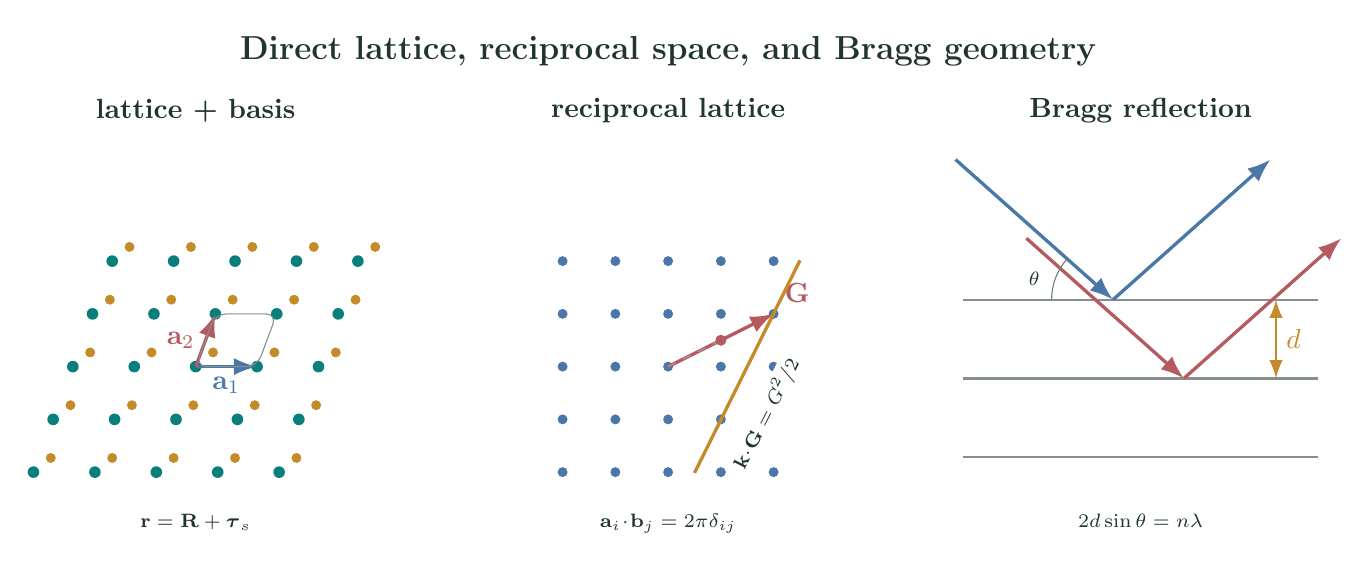
\begin{tikzpicture}[font=\sffamily,text=ink,>=Latex]
  \node[font=\bfseries\large] at (0,4.25) {Direct lattice, reciprocal space, and Bragg geometry};
  \begin{scope}[xshift=-6.0cm,yshift=.25cm]
    \node[font=\bfseries] at (0,3.25) {lattice + basis};
    \foreach \i in {-2,-1,0,1,2}
      \foreach \j in {-2,-1,0,1,2}{
        \fill[teal] (0.78*\i+0.25*\j,0.67*\j) circle (2.1pt);
        \fill[gold] (0.78*\i+0.25*\j+0.22,0.67*\j+0.18) circle (1.8pt);
      }
    \draw[->,very thick,blue] (0,0)--(.78,0) node[midway,below] {$\mathbf a_1$};
    \draw[->,very thick,rose] (0,0)--(.25,.67) node[midway,left] {$\mathbf a_2$};
    \draw[rounded corners,ink!55] (0,0)--(.78,0)--(1.03,.67)--(.25,.67)--cycle;
    \node[font=\scriptsize,anchor=north] at (0,-1.75) {$\mathbf r=\mathbf R+\boldsymbol\tau_s$};
  \end{scope}
  \begin{scope}[yshift=.25cm]
    \node[font=\bfseries] at (0,3.25) {reciprocal lattice};
    \foreach \i in {-2,-1,0,1,2}
      \foreach \j in {-2,-1,0,1,2}
        \fill[blue] (0.67*\i,0.67*\j) circle (1.8pt);
    \draw[->,very thick,rose] (0,0)--(1.34,.67) node[above right] {$\mathbf G$};
    \draw[gold,very thick] (.335,-1.35)--(1.675,1.35);
    \node[font=\scriptsize,rotate=63,fill=white,inner sep=1pt] at (1.25,-.6)
      {$\mathbf k\!\cdot\!\mathbf G=G^2/2$};
    \draw[dashed,ink!45] (0,0)--(.67,.335);
    \fill[rose] (.67,.335) circle (2pt);
    \node[font=\scriptsize,anchor=north] at (0,-1.75) {$\mathbf a_i\!\cdot\!\mathbf b_j=2\pi\delta_{ij}$};
  \end{scope}
  \begin{scope}[xshift=6.0cm,yshift=.25cm]
    \node[font=\bfseries] at (0,3.25) {Bragg reflection};
    \foreach \y in {-1.15,-.15,.85}{\draw[ink!55,thick] (-2.25,\y)--(2.25,\y);}
    \coordinate (P) at (-.35,.85);
    \coordinate (Q) at (.55,-.15);
    \draw[blue,very thick,->] ($(P)+(-2.0,1.78)$)--(P);
    \draw[blue,very thick,->] (P)--($(P)+(2.0,1.78)$);
    \draw[rose,very thick,->] ($(Q)+(-2.0,1.78)$)--(Q);
    \draw[rose,very thick,->] (Q)--($(Q)+(2.0,1.78)$);
    \draw[<->,gold,thick] (1.72,-.15)--(1.72,.85) node[midway,right] {$d$};
    \draw[ink!65] ($(P)+(-.78,0)$) arc[start angle=180,end angle=138,radius=.78];
    \node[font=\scriptsize] at (-1.35,1.12) {$\theta$};
    \node[font=\scriptsize,anchor=north] at (0,-1.75) {$2d\sin\theta=n\lambda$};
  \end{scope}
\end{tikzpicture}
\end{document}
